%Chapter 7
\chapter{Formalism of Quantum Mechanics Part 2}
So far we have described a quantum mechanical system by a state $|\Psi\rangle$ in the Hilbert space H and its time evolution by the Schr¨odinger equation $i\hbar\partial_t|\Psi(t)\rangle=H|\Psi(t)\rangle$. This description assumes that at a time $t = t_0$ the state $|\Psi\rangle$ is known as a 1-dim vector in $\mathcal{H}$. This can be generated, for example, by measuring a complete set of observables; for the particle in the central potential by determining $E, L^2$ and $L_z$, for the H atom ($e ^-$ with spin), the measurement of $E, L^2$ and $L_z$ is no longer sufficient (because of the $SO (4)$ symmetry). \\\\In general, we can imagine situations where we can not maximize the system so that we can not specify a state vector in $\mathcal{H}$ as the starting value. This is the case, for example, with an effusion cell, see figure 7.1: the simple opening (without channel) produces particles with impulses $\vec{p}$ in all directions ($p_x> 0$) and different energies. How should such a weakly prepared system be described?
%图 7.1
\begin{figure}[ht]
    \begin{minipage}{0.6\textwidth}
        \centering
        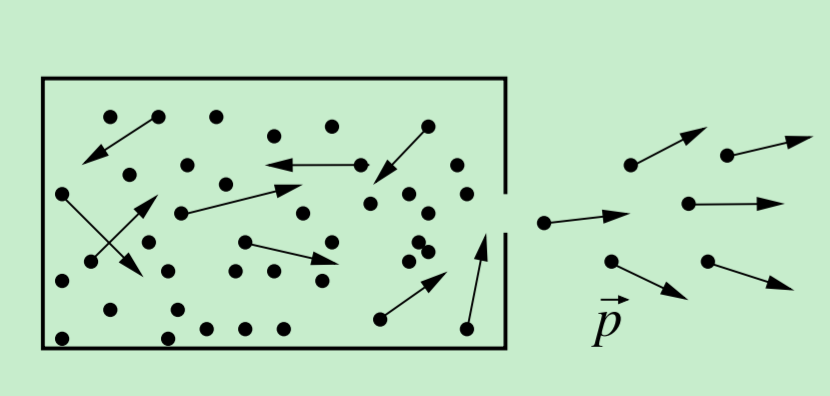
\includegraphics[scale=1]{7_1.PNG}
    \end{minipage}
    \begin{minipage}{0.4\textwidth}
        \captionsetup{font={Large}}
        \caption{The effusion cell produces an ensemble of particles with different impulse directions $\vec{p}$ and different (thermally distributed) energies.}
    \end{minipage}
\end{figure}

\section{Density matrix as a statistical operator}
A clean physical characterization of the system requires that we have the adequate information at our disposal. This information is the classical-statistical (incoherent) information underlying the preparation. Transferred to the Hilbert space $\mathcal{H}$, this information gives us the probability that a state $|\Psi\rangle\in H$ occurs. In the example of the effusion cell, this information is given by the distribution of the pulses $\vec{p}$ in the cell; it allows us to calculate the distribution of the momentum in the beam as long as we know the geometry of the opening. We can then give the following classical description of the system:
\begin{enumerate}
    \item[] The (1-dim) state $|\Psi_i\rangle$ is realized in the prepared ensemble with the probability $p_i \leq 1$.
\end{enumerate}
The measurement of any observable $A$ should then be by the expected value

%公式 7.1
\begin{equation}
    \langle A\rangle=\sum_{i} p_{i}\left\langle\Psi_{i}|A| \Psi_{i}\right\rangle
    \end{equation}
be given. We want to put this expression into a generic form. Let $\{\varphi_i\}$ be a complete orthonormal system, then we can print $\langle A\rangle$ by $A$ and the density matrix $\rho$,
%公式 7.2
\begin{equation}
\begin{aligned}\langle A\rangle &=\sum_{i} p_{i}\left\langle\Psi_{i}|A| \Psi_{i}\right\rangle \\ &=\sum_{i} p_{i}\left\langle\Psi_{i} | \varphi_{m}\right\rangle\left\langle\varphi_{m}|A| \varphi_{n}\right\rangle\left\langle\varphi_{n} | \Psi_{i}\right\rangle \\ &=\sum_{m, n}\left\langle\varphi_{m}|A| \varphi_{n}\right\rangle\left\langle\varphi_{n}\left|\sum_{i} p_{i}\right| \Psi_{i}\right\rangle\left\langle\Psi_{i} | \varphi_{m}\right\rangle \\ &=\sum_{m}\left\langle\varphi_{m}|A \rho| \varphi_{m}\right\rangle \\ &=\operatorname{Trace}(A \rho) \end{aligned}
\end{equation}
The maximum information about the system is thus in the density matrix $\rho$,
%公式 7.3
\begin{equation}
    \rho=\sum_{i} p_{i}\left|\Psi_{i}\right\rangle\left\langle\Psi_{i}\right|=\sum_{i} p_{i} \underbrace{P_{i}}_{\text {Projector }}
    \end{equation}
because with their help we can calculate the result of each measurement. Here $p_i\leq 1$, $\sum_i p_i = 1$ and the states are normalized to $||\Psi_i||=1$. We distinguish between pure and mixed states:
%公式 7.4
\begin{equation}
\begin{aligned} \text { pure condition } & \rightarrow \rho=|\Psi\rangle\langle\Psi| \\ \text { mixed condition } & \rightarrow \rho=\sum_{i} p_{i}\left|\Psi_{i}\right\rangle\left\langle\Psi_{i}\right| \quad \text { mit } \quad p_{i}<1 \forall i \end{aligned}
\end{equation}
The important point here is the coherence: Every ray $|\Psi_i\rangle$ corresponds to a coherent state-these states are incoherently superposed in $\rho$ with probabilities $p_i$. The best way to understand this is to print the density matrix $\rho$ in a basis {$\varphi_i$} and then calculate $\langle A\rangle$. Let $|\Psi_i\rangle=\sum_j c_{ij}|\varphi_j\rangle$, then
%公式 7.5
\begin{equation}
\begin{aligned} \rho &=\sum_{i} p_{i}\left|\Psi_{i}\right\rangle\left\langle\Psi_{i}\right| \\ &=\sum_{i j k} p_{i} c_{i j} c_{i k}^{*}\left|\varphi_{j}\right\rangle\left\langle\varphi_{k}\right| \end{aligned}
\end{equation}
%公式 7.6
\begin{equation}
\begin{aligned}\langle A\rangle &=\operatorname{Trace}(A \rho)=\sum_{m}\left\langle\varphi_{m}\left|A \sum_{i j k} p_{i} c_{i j} c_{i k}^{*}\right| \varphi_{j}\right\rangle \underbrace{\left\langle\varphi_{k} | \varphi_{m}\right\rangle}_{\delta_{k m}} \\ &=\sum_{i j m} p_{i} c_{i j} c_{i m}^{*}\left\langle\varphi_{m}|A| \varphi_{j}\right\rangle \end{aligned}
\end{equation}
The coefficients $p_i$ (probabilities) and $c_{ij}$ (amplitudes) of the incoherent and the coherent sum are completely different. In (7.6), the $0 \leq p_i \leq 1$ are real probabilities, while the $c_{ij}\in\mathbb{C}$ are complex amplitudes. The phase relation among the $c_{ij}$ as a consequence of the coherent superposition of $|\varphi_j\rangle$ to $|\Psi_i\rangle$ is clearly evident in the result. In the incoherent sum over the ¨$p_i$ no such phases occur.\\\\
The density matrix $\rho$ has some nice properties:
%列表
\begin{enumerate}
    \item[-] $\rho=\rho^{\dagger} \text { is hermitian, } p_{i} \in \mathbb{R} \text { and } P_{i}=\left|\Psi_{i}\right\rangle\left\langle\Psi_{i}\right| \text {are}$ 
    \item[]$\text{hermitean projection operators.}$.
    \item[-] $\rho \text { is definitely positive, there is }\langle\varphi|\rho| \varphi\rangle=\sum_{i} p_{i}\left|\left\langle\varphi | \Psi_{i}\right\rangle\right|^{2}  \geq 0$ 
    \item[-] $\operatorname{Trace}[\rho]=1, \text{there is } \sum_{n}\left\langle\varphi_{n}|\rho| \varphi_{n}\right\rangle=\sum_{i, n} p_{i}\left|\left\langle\varphi_{n} | \Psi_{i}\right\rangle\right|^{2}$ 
    \item[] $=\sum_{i} p_{i}\left\langle\Psi_{i}\right| \overbrace{\sum_{n}\left|\varphi_{n}\right\rangle\left\langle\varphi_{n}\right\rangle}^{\|}=\sum_{i} p_{i}=1 \text { ist. }$ 
    \item[-] $\text{For a pure state is}\rho=P=|\Psi\rangle\langle\Psi| \text{ an projector } \rho^{2}=\rho$.
     
    \item[-] $\text{Trace}[\rho^2]=\left\{
        \begin{array}{ll}
            1, & \text{pure condition},\\
            <1, & \text{mixed condition},
        \end{array} 
        \right.$
    \item[] $\operatorname{because} \rho^{2}=\sum_{i} p_{i}^{2}\left|\Psi_{i}\right\rangle\left\langle\Psi_{i}\right|, \text { and } \operatorname{Trace}\left[\rho^{2}\right]=\sum_{i} p_{i}^{2}$ 
\end{enumerate}
Finally, we still need the time evolution for the density matrix $\rho$: the time evolution of the states is given by the Schr¨odinger equation (SG),
%公式 7.7
\begin{equation}
\begin{aligned} i \hbar \partial_{t}\left|\Psi_{i}(t)\right\rangle &= H\left|\Psi_{i}(t)\right\rangle \\- i \hbar \partial_{t}\left\langle\Psi_{i}(t)\right| &=\left\langle\Psi_{i}(t)\right| H \end{aligned}
\end{equation}
with which we can calculate the time evolution of $\rho$,

%公式 7.8
\begin{equation}
\begin{aligned} i \hbar \partial_{t} \rho &=\sum_{i} p_{i}\left(\overbrace{\left(i \hbar \partial_{t}\left|\Psi_{i}\right\rangle\right)}^{H\left|\Psi_{i}\right\rangle}\left\langle\Psi_{i}|+| \Psi_{i}\right\rangle \overbrace{\left(i \hbar \partial_{t}\left\langle\Psi_{i}\right|\right)}^{-\left\langle\Psi_{i}\right| H}\right) \\ &=H \rho-\rho H=[H, \rho] \end{aligned}
\end{equation}
Formula (7.8) is the von Neumann differential equation for the density matrix, the quantum mechanical analogue to the Liouville equation in (classical) statistical mechanics (time evolution in phase space).

\section{Dynamic Pictures: Schr¨odinger - Heisenberg - Dirac}
\subsection{Schr¨odinger image}
The Schr¨odinger picture is the picture we used so far: 
\begin{enumerate}
    \item[-] The state vectors $|\Psi(t)\rangle$ are time-dependent,
    \item[-] The operators $A$ are time-independent,
    \item[-] The time dependency of the states $|\Psi(t)\rangle$ is given by the Schr¨odinger equation, 
\end{enumerate}

%公式 7.9
\begin{equation}
    i \hbar \partial_{t}|\Psi(t)\rangle= H|\Psi(t)\rangle, \quad\left|\Psi\left(t_{0}\right)\right\rangle=\left|\Psi_{0}\right\rangle
    \end{equation}
We introduced the time evolution operator ¨$U (t, t_0)$, so that
% 7.10
\begin{equation}
    |\Psi(t)\rangle= U\left(t, t_{0}\right)\left|\Psi\left(t_{0}\right)\right\rangle
    \end{equation}
The operator $U$ should get the norm (preservation of the probability), which implies its unitarity
%公式 7.11

\begin{align}\langle\Psi(t) \Psi(t)\rangle &=\left\langle\Psi_{0} \Psi_{0}\right\rangle \\ & \Rightarrow U^{\dagger}\left(t, t_{0}\right) U\left(t, t_{0}\right)=\mathbb{I} \\ U^{-1}\left(t, t_{0}\right) &=U^{\dagger}\left(t, t_{0}\right) 
\end{align}
%公式 12
%公式 13
Further, from $|\Psi(t=t_0)\rangle=|\Psi_0\rangle$, it follows that $U (t_0, t_0) = \mathbb{I}$ is the identity. The time evolution from $t_0$ to $t$ via $t_1$ is independent of $t_1$ and multiplicative, hence
%公式 14

\begin{align} U\left(t, t_{0}\right) &=U\left(t, t_{1}\right) U\left(t_{1}, t_{0}\right) \\ \stackrel{t=t_{0}}{\Rightarrow} U^{-1}\left(t, t_{0}\right) &=U\left(t_{0}, t\right) \stackrel{(7,13)}{=} U^{\dagger}\left(t, t_{0}\right) 
\end{align}
%公式 15
In closed (conservative) systems, no point in time is excellent, and so we get the translation invariant form
%公式 16
\begin{equation}
    U\left(t, t_{0}\right)=U\left(t-t_{0}\right)
    \end{equation}
Finally, the Schr¨odinger equation (7.9) implements the differential equation for ¨$U$,

%
\begin{equation}
    i \hbar \partial_{t} U\left(t, t_{0}\right)=H U\left(t, t_{0}\right)
    \end{equation}
For $\partial_t H = 0$ we can integrate (7.17) immediately
%公式 18
\begin{equation}
    U\left(t, t_{0}\right)=e^{-i H\left(t-t_{0}\right) / \hbar}
    \end{equation}
in fact, $U (t_0, t_0) = \mathbb{I}, U$ is unitary, multiplicative, and dependent only on $t - t_0$. The Hamiltonian $H$ is the infinitesimal generator of time evolution (time translation) and with $H$ hermitesch, $U$ is also unitary, as expected.\\\\
In the general case with $\partial_t H\neq 0$ we have to do something more: we can formally integrate (7.17) and then solve iteratively,
%公式 19
\begin{align}
    U\left(t, t_{0}\right)&=\mathbb{I}+\frac{1}{i \hbar} \int_{t_{0}}^{t} d t^{\prime} H\left(t^{\prime}\right) U\left(t^{\prime}, t_{0}\right),\\
    &\approx \mathbb{I}+ \frac{1}{i\hbar}\int_{t_0}^t dt_1H(t_1)+\frac{1}{(i\hbar)^2}\int_{t_0}^t dt_1\int_{t_0}^{t_1}dt_2H(t_1)H(t_2)+\cdots,\nonumber\\
    &=\mathbb{I}+\sum_{n=1}^{\infty}U^{(n)}(t,t_0),\\
    U^{(n)}(t,t_0)&=\left(\frac{1}{i\hbar}\right)^n\int_{t_0}^t dt_1\int_{t_0}^{t_1}dt_2\cdots\int_{t_0}^{t_{n-1}}dt_nH(t_1)H(t_2)\cdots H(t_n),\nonumber
\end{align}
%公式 20
and we get the von Neumann series. Important in (7.20) is that there is a time order: $t\geq t_1\geq t_2\geq\cdots\geq t_0$,
%公式 21
\begin{equation}
\begin{array}{cccc}
    {H\left(t_{1}\right)} & {\cdots} & {H\left(t_{n}\right)} & \\ 
    {\uparrow} & {} & {\uparrow} & \\ 
    {\text { latter }} & {} & {\text { earlier }} & {\text { times }}
\end{array}
\end{equation}
This time order is unpleasant but formally remediable: The time-order implies an integration over the part ¨$t\geq t_1\cdots \geq t_n \geq t_0$ of the hypercube in $\mathbb{R}^n$, cf. figure 7.2 for ¨$n = 2$.
%图 7.2
\begin{figure}[ht]
    \begin{minipage}{0.5\textwidth}
        \centering
        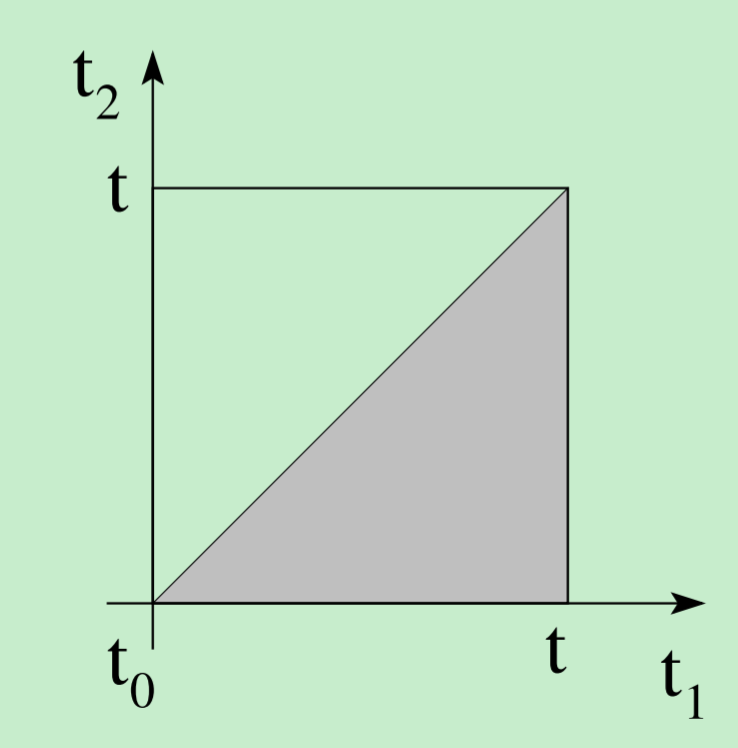
\includegraphics[scale=1]{7_2.PNG}
    \end{minipage}
    \begin{minipage}{0.5\textwidth}
        \captionsetup{font={Large}}
        \caption{Integration area (hatched in gray) over the time-ordered sector for the case $n = 2$.}
    \end{minipage}
\end{figure}
\\
As a formal tool, we define the timing operator $T$, which times a sequence of time-dependent operators,

%公式 22
\begin{equation}
T A\left(t_{1}\right) B\left(t_{2}\right)=\left\{\begin{array}{ll}{A\left(t_{1}\right) B\left(t_{2}\right)} & {: t_{1}>t_{2}} \\ {B\left(t_{2}\right) A\left(t_{1}\right)} & {: t_{2}>t_{1}}\end{array}\right.
\end{equation}
the generalization to $n$ operators is trivial,
%公式 23
\begin{equation}
    T \prod_{i=1}^{n} A_{i}\left(t_{i}\right)=A_{\pi_{1}}\left(t_{\pi_{1}}\right) \ldots A_{\pi_{n}}\left(t_{\pi_{n}}\right)
    \end{equation}
with $\pi\in S_n, S_n$ is the symmetric group (group of permutations), $\Pi$ is the permutation which orders the times, $t_{\pi_1}\geq t_{\pi_2}\geq \cdots \geq t_{\pi_n}$. The timing operator $T$ allows us to extend the integrals in (7.20) to the full cube, for ¨$n = 2$,
%公式 24
\begin{equation}
\begin{aligned} \int_{t_{0}}^{t} d t_{1} \int_{t_{0}}^{t_{1}} d t_{2} H\left(t_{1}\right) H\left(t_{2}\right)=& \frac{1}{2}\left(\int_{t_{0}}^{t} d t_{1} \int_{t_{0}}^{t_{1}} d t_{2} H\left(t_{1}\right) H\left(t_{2}\right)\right.\\ &\left.+\int_{t_{0}}^{t} d t_{2} \int_{t_{0}}^{t_{2}} d t_{1} H\left(t_{2}\right) H\left(t_{1}\right)\right) \\=& \frac{1}{2} \int_{t_{0}}^{t} d t_{1} \int_{t_{0}}^{t} d t_{2} T H\left(t_{1}\right) H\left(t_{2}\right) \end{aligned}
\end{equation}
and for any $n$,

% 25
\begin{equation}
    \int_{t_{0}}^{t} d t_{1} \int_{t_{0}}^{t_{1}} d t_{2} \cdots \int_{t_{0}}^{t_{n-1}} d t_{n}=\frac{1}{n !} \prod_{i=1}^{n} \int_{t_{0}}^{t} d t_{i} T
    \end{equation}
That's how we get
%公式 26
\begin{equation}
    U^{(n)}\left(t, t_{0}\right)=\frac{1}{n !}\left(\frac{1}{i \hbar}\right)^{n} \int_{t_{0}}^{t} d t_{1} \ldots \int_{t_{0}}^{t} d t_{n} T H\left(t_{1}\right) \ldots H\left(t_{n}\right)
    \end{equation}
and we can (at least formally) explicitly state the time evolution operator $U$ in the Schr¨odinger image,
% 27
\begin{equation}
    U\left(t, t_{0}\right)=T \exp \left[-\frac{i}{\hbar} \int_{t_{0}}^{t} d t^{\prime} H\left(t^{\prime}\right)\right]
    \end{equation}
Note that (7.27) is always the series (7.20), with $U^{(n)}$ given by (7.20) or (7.26) with $T$ defined in (7.23).\\\\
In some cases the time-evolution operator is simplified: If $[H (t), H (t')] = 0$ we can set $T = \mathbb{I}$ and (7.27) becomes

% 28
\begin{equation}
    U\left(t, t_{0}\right)=\exp \left[-\frac{i}{\hbar} \int_{t_{0}}^{t} d t^{\prime} H\left(t^{\prime}\right)\right] \quad \Leftarrow \quad\left[H(t), H\left(t^{\prime}\right)\right]=0
    \end{equation}
It gets even easier if $\partial_tH = 0$,
%公式 29
\begin{equation}
    U\left(t, t_{0}\right)=\exp \left[-\frac{i}{\hbar} H\left(t-t_{0}\right)\right] \quad \Leftarrow \partial_{t} H=0
    \end{equation}
\subsection{Heisenberg picture}
In the Heisenberg picture we roll the time evolution from the states to the operators. Relevant are the (measurable) expectation values ​​$\langle A\rangle$, which should remain invariant,
%公式 30
\begin{equation}
    U\left(t, t_{0}\right)=\exp \left[-\frac{i}{\hbar} H\left(t-t_{0}\right)\right] \quad \Leftarrow \partial_{t} H=0
    \end{equation}
In the Heisenberg picture are the
%
$$
\begin{array}{ll}{-\text { conditions }} & {\left|\Psi_{H}\right\rangle=\left|\Psi\left(t_{0}\right)\right\rangle=\left|\Psi_{0}\right\rangle \quad \text { independent of time }} \\ {-\text { operators }} & {A_{H}(t)=U^{\dagger}\left(t, t_{0}\right) A U\left(t, t_{0}\right) \quad \text { time-dependent. }}\end{array}
$$
The equation of motion now applies to the operators and reads
%公式 31
\begin{equation}
\begin{aligned} i \hbar \frac{d}{d t} A_{H}(t) &=\underbrace{\left(i \hbar \partial_{t} U^{\dagger}\right)}_{-(H U)^{\dagger}} A U+U^{\dagger} A \underbrace{i \hbar \partial_{t} U}_{H U}+\underbrace{U^{\dagger} i \hbar \partial_{t} A U}_{\text {def }: i \hbar \partial_{t} A_{H}} \\ &=-(H U)^{\dagger} A U+U^{\dagger} A H U+i \hbar \partial_{t} A_{H} \\ &=\left[A_{H}, H_{H}\right]+i \hbar \partial_{t} A_{H} \end{aligned}
\end{equation}
If $\partial_tH = 0$ then $[H, U] = 0$ and thus $H_H (t) \equiv H_H = H$. In the conservative case, $H_H = H$ is time-independent, while other operators are the dynamics
%公式 32
\begin{equation}
    A_{H}(t)=\mathrm{e}^{i H\left(t-t_{0}\right) / \hbar} A \mathrm{e}^{-i H\left(t-t_{0}\right) / \hbar}
    \end{equation}
to have. Instead of the rotation of the vectors in the Hilbert space $\mathcal{H}$ (note: $U$ is unitary $\Rightarrow ||\Psi||$ and $\langle \Phi,\Psi\rangle$ are obtained under time evolution), we now have a rotation of the operators in the opposite direction (the relative motion of $|\Psi\rangle$ and $A$ remains the same ). For the motion constants, the following applies:
%公式 33
\begin{equation}
    A_{H} \text { a motion constant } \Leftrightarrow \partial_{t} A=0,\left[H_{H}, A_{H}\right]=0
    \end{equation}
Note that not only expectation hAi but also angles $\langle\Phi_H,\Psi_H\rangle=\langle\Phi(t),\Psi(t)\rangle$ are obtained. For the permutation relations applies
%公式 34
\begin{equation}
    [A, B]=C \quad \Rightarrow \quad\left[A_{H}, B_{H}\right]=C_{H}
    \end{equation}
because $[A_H, B_H] = U^{\dagger}AUU^{\dagger}BU-U^{\dagger}BUU^{\dagger}AU=U^{\dagger}[A,B]U=U^{\dagger}CU=C_H$.\\\\
Although the Schr¨odinger picture is conceptually simpler, the Heisenberg picture is more consistent, since the relation to classical physics via correspondence is more direct:
\begin{enumerate}
    \item[] $|\Psi_H\rangle\hat{=}$ orbit in phase space = total info. from preparation,
    \item[] $A_H (t) \hat{=}$ phase space function $A [q (t), p (t), t]$, dynamic variable. 
\end{enumerate}
Finally, let's look at the (practical) Dirac image:
\subsection{Dirac or interaction image}
Consider (7.20); if $H$ were small then we could break off the series as an approximation and get a good result. Usually, however, $H$ is not small. On the other hand, $H$ often consists of a simple, soluble fraction H0 and a correction $ H_0$, e.g.
\begin{enumerate}
    \item[-] $H_0$ = free particle or time independent,
    \item[-] $H'$ = interaction or time-dependent disturbance 
\end{enumerate}
In the interaction picture (WW image) we want to have the evolution (7.20) for $H'$ instead of $H$; it turns out that the corresponding evolutionary operator in the Dirac image is given by
%公式 35
\begin{equation}
    U_{D}\left(t, t_{0}\right)=\underbrace{U_{0}^{\dagger}\left(t, t_{0}\right)}_{\text {inverse free dynamics.  }}\underbrace{U(t,t_0)}_{\text{full dynamics}}
    \end{equation}
To do this, we distribute the dynamics in the Dirac image to states and operators,
%公式 36
\begin{equation}
\begin{aligned}\langle A\rangle &=\langle\Psi(t)|A| \Psi(t)\rangle \\ &=\left\langle\Psi_{0}\left|U^{\dagger}\left(t, t_{0}\right) A U\left(t, t_{0}\right)\right| \Psi_{0}\right\rangle \\ &=\underbrace{\left\langle\Psi_{0}\right| U^{\dagger}\left(t, t_{0}\right) U_{0}\left(t, t_{0}\right)}_{\left\langle\Psi_{D}(t)\right|} \underbrace{U_{0}^{\dagger}\left(t, t_{0}\right) A U_{0}\left(t, t_{0}\right)}_{A_{D}(t)} \underbrace{U_{0}^{\dagger}\left(t, t_{0}\right) U\left(t, t_{0}\right)\left|\Psi_{0}\right\rangle}_{\left|\Psi_{D}(t)\right\rangle} \\ &=\left\langle\Psi_{D}(t)\left|A_{D}(t)\right| \Psi_{D}(t)\right\rangle \end{aligned}
\end{equation}
Thus, the simple part of the dynamics is in the operators; with $\partial_tH_0 = 0$
%公式 37
\begin{equation}
    A_{D}(t)=e^{i H_{0}\left(t-t_{0}\right) / \hbar} A e^{-i H_{0}\left(t-t_{0}\right) / \hbar}
    \end{equation}
while the remaining (difficult but hopefully small) part of the dynamics is in $\Psi_D (t)$,
%公式 38
\begin{equation}
\begin{aligned} \Psi_{D}(t) &=U_{D}\left(t, t_{0}\right) \Psi_{0} \\ \text{with } U_{D}\left(t, t_{0}\right) &=U_{0}^{\dagger}\left(t, t_{0}\right) U\left(t, t_{0}\right) \end{aligned}
\end{equation}
The remaining time evolution operator $U_D$ obeys the differential equation
%公式 39
\begin{equation}
\begin{aligned} i \hbar \partial_{t} U_{D} &=i \hbar \partial_{t}\left[e^{i H_{0}\left(t-t_{0}\right) / \hbar} U\right] \\ &=U_{0}^{\dagger} \underbrace{\left(-H_{0}+H\right)}_{H^{\prime}} U \underbrace{U_{0}^{\dagger} U}_{U_{D}} \\ &=H_{D}^{\prime} U_{D} \end{aligned}
\end{equation}
with
%公式 40
\begin{equation}
    H_{D}^{\prime}=\mathrm{e}^{i H_{0}\left(t-t_{0}\right) / \hbar} H^{\prime} \mathrm{e}^{-i H_{0}\left(t-t_{0}\right) / \hbar}
    \end{equation}
By iteration, we obtain the following series as already known from the Schr¨odinger picture (see (7.20)),
%公式 41

\begin{align} 
    U_{D}\left(t, t_{0}\right)=& 11+\left(\frac{1}{i \hbar}\right) \int_{t_{0}}^{t} d t_{1} H_{D}^{\prime}\left(t_{1}\right)+\nonumber\\ 
    & \vdots \nonumber\\ 
    &+\frac{1}{n !}\left(\frac{1}{i \hbar}\right)^{n} \int_{t_{0}}^{t} d t_{1} \ldots d t_{n} T H_{D}^{\prime}\left(t_{1}\right) \ldots H_{D}^{\prime}\left(t_{n}\right)\\ 
    &=T \exp \left[-\frac{i}{\hbar} \int_{t_{0}}^{t} d t^{\prime} H_{D}^{\prime}\left(t^{\prime}\right)\right]
\end{align}
%公式 42
\section{Time reversal $T$}
In the context of this formal chapter we deal with another important symmetry, time reversal. We define the time reversal operator $\mathcal{T}$. Let $\mathcal{T}$ be a symmetry of the (closed) system. Thus, with $\Psi_E$, an eigenvector to H with the eigenvalue $E, \mathcal{T} \Psi_E$ is also an eigenvector to $E$. The question arises whether $\mathcal{T}\Psi_E$ is parallel to $\Psi_E$ or a new eigenvector to $E$ of $H$, the time reversal invariance implies a doubling of the Degeneracy or not. The answer is given by the Frobenius-Schur test:
\\\\
Let $G$ be the symmetry group of the operator $A$, let $A$ be invariant under time reversal. Consider the degenerations of the eigenspaces of $A$ defined by $G$; these are given by the dimensions of the associated irreducible representations $\mathcal{D}^{\alpha}_G$. The eigenspace to $\mathcal{D}^{\alpha}_G$ is doubled due to the time reversal invariance of $A$ if $FS\equiv\sum_{a\in G}\mathcal{X}^{\alpha}_G(a^2)$ or $-g$, where $\mathcal{X}^{\alpha}_G$ is the character of the representation $\mathcal{D}^{\alpha}_G$ and $g$ denotes the order of the group $G$. If $F S = g$, the degeneracy remains unchanged. These results apply to spineless particles.\footnote{For spin-1/2 particles, the degeneracy is doubled if ¨$F S = g, 0$, whereas the degeneracy remains unchanged for $F S = -g$. Known in this context is the Kramer's degeneration, dim $\operatorname{Eig}^E_H \geq 2$ for spin-1/2 particles.}
\\\\
In the following, we consider some properties of time reversal $\mathcal{T}$, in particular their representation in space. Let $\Psi$ be an arbitrary state in Hilbert space. We use the eigenbasis $\{\Psi_E\}$ for $H$ and develop $\Psi$ in the $\Psi_E$,
%公式 43
\begin{equation}
    \Psi=\sum_{E} a_{E} \Psi_{E}
    \end{equation}
We perform the following operation with $\Psi$, cf. figure 7.3,
%图 7.3
\begin{figure}[ht]
    \begin{minipage}{0.6\textwidth}
        \centering
        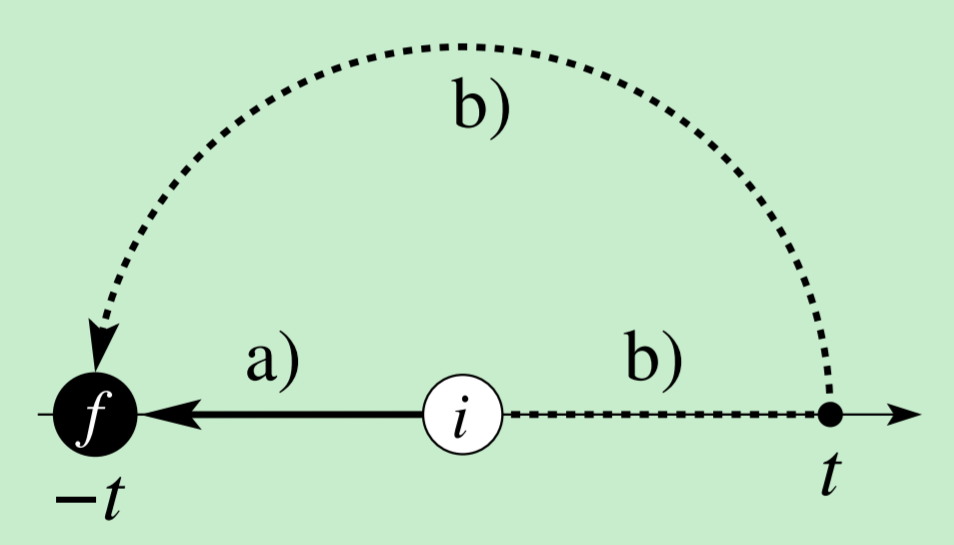
\includegraphics[scale=1]{7_3.PNG}
    \end{minipage}
    \begin{minipage}{0.4\textwidth}
        \captionsetup{font={Large}}
        \caption{Time reversal and propagation. The routes $a)$ and $b)$ generate the same final state $f$ from the same initial state $i$.}
    \end{minipage}
\end{figure}
\begin{enumerate}
    \item[a)] first time reversal, then propagation in $-t$ (ie $U_{-t}\mathcal{T}\Psi$),
    \item[b)] first propagation in $t$, then time reversal (ie $\mathcal{T}U_t\Psi$).
\end{enumerate}
a) and b) give only the same result if $\mathcal{T}$ is antilinear, that is, it must be valid
%公式 44
\begin{equation}
    \mathcal{T}(a \Psi+b \Phi)=a^{*} \mathcal{T} \Psi+b^{*} \mathcal{T} \Phi
    \end{equation}
Then we find for the ways a) and b):
%公式 45
\begin{align}
    \text { a) } & \quad \sum_{E} e^{i E t / \hbar} a_{E}^{*} \mathcal{T} \Psi_{E}\nonumber\\
    \text { b) } & \quad \mathcal{T} \sum_{E} e^{-i E t / \hbar} a_{E} \Psi_{E}=\sum_{E} e^{i E t / \hbar} a_{E}^{*} \mathcal{T} \Psi_{E}
\end{align}
Now consider the time reversal of the Schr¨odinger equation (we apply $\mathcal{T}$ to the equation of the equation)

%公式 46
\begin{equation}
\begin{array}{rcl} 
    i \hbar \partial_{t} \Psi &=&H \Psi \\
    &\downarrow&\\
    -i \hbar \partial_{t} \mathcal{T} \Psi &=&\mathcal{T} H \Psi \\ 
    & \downarrow& \text { falls } \mathcal{T} \text { is a symmetry } \\ 
    &=&H \mathcal{T} \Psi \end{array}
\end{equation}
So if $[H, \mathcal{T}] = 0$, then ¨$\mathcal{T}\Psi$ satisfies the Schr¨odinger equation with $t \rightarrow -t$, as expected.
\\
We want to find a representation of $\mathcal{T}$ (without spin): the position $\vec{r}$ should be invariant below $\mathcal{T}$, the linear and angular momenta should be inverted, then we have
%公式 47

%公式 48

\begin{align}{\vec{r} \mathcal{T}\;=\;} & {\mathcal{T} \vec{r} \quad \Rightarrow \quad[\vec{r}, \mathcal{T}]\;=\;0} \\ {\vec{p} \mathcal{T}\;=\;} & {-\mathcal{T} \vec{p}} \\ {\vec{L} \mathcal{T}\;=\;} & {-\mathcal{T} \vec{L}}\end{align}
\\
%公式 49
In the positional representation, $\vec{r}=\vec{r},\vec{p}=-i\hbar\nabla$, and we can give a simple representation for $\mathcal{T}$ such that $\mathcal{T}$ is antilinear and (7.47) - (7.49) are satisfied,
%公式 50
\begin{equation}
    \mathcal{T} \Psi=\Psi^{*}, \quad \text { complex conjugation. }
    \end{equation}
This representation of $\mathcal{T}$ is valid only in the Ortsdarstellung.\footnote{For a spin-1/2 particle described by the spinor $\Psi=\left(\begin{array}{c}{\mathcal{X}_{\uparrow}} \\ {\mathcal{X}_{\downarrow}}\end{array}\right)$ is the representation given by $\mathcal{T}\Psi=i\sigma_y\Psi^*=\left(\begin{array}{c}{\mathcal{X}^*_{\downarrow}}\\{-\mathcal{X}^*_{\uparrow}}\end{array}\right)$ and it is $\mathcal{T}^2\Psi = -\Psi$.}
Proof: We show that the representation (7.50) is determined to a factor $f = \pm 1$:
%列表
\begin{enumerate}
    \item[i)] $ {\hat{\mathcal{T}}|x\rangle= f(x)|x\rangle, \text{with } f(x) \in \mathbb{C}, \text{because } \hat{x} \hat{\mathcal{T}}|x\rangle=\hat{\mathcal{T}} \hat{x}|x\rangle= x \hat{\mathcal{T}}|x\rangle} {\text { and that}}$
    \item[] ${\text{is why } \hat{\mathcal{T}}|x\rangle \propto|x\rangle}$
    \item[ii)]$\hat{\mathcal{T}}|p\rangle=g(p)|-p\rangle, \text{ with }g(p)\in\mathbb{C}$ 
    \item[iii)] $f \;\&\; g$ are constants, because\\
        $\begin{aligned} \qquad\hat{\mathcal{T}}|p\rangle &=\hat{\mathcal{T}} \sum_{x}\langle x | p\rangle|x\rangle \\ &=\hat{\mathcal{T}} \sum_{x} e^{-i p x}|x\rangle=\sum_{x} e^{i p x} \hat{\mathcal{T}}|x\rangle=\sum_{x} f(x) e^{i p x}|x\rangle \\ &= g(p)|-p\rangle= g(p) \sum_{x} e^{i p x}|x\rangle \end{aligned}$
    \item[] and we receive $g(p)e^{ipx}=e^{ipx}f(x)$ and thus $f=g=\text{const}.\in\mathbb{C}$
    \item[iv)] We write the state $|\Psi\rangle$ in the location view, ,
    \item[] $|\Psi\rangle=\sum_x \psi(x)|x\rangle$ and calculate the effect of $\hat{\mathcal{T}}$, 
    \item[] $\qquad\qquad \hat{\mathcal{T}}|\Psi\rangle=\sum_{x} \psi^{*}(x) f|x\rangle= f \sum_{x} \psi^{*}(x)|x\rangle$
    \item[] is also $[\hat{\mathcal{T}}\Psi](y)=f\Psi^*(y).$
    \item[v)] Finally is $\hat{\mathcal{T}}^{2}=\mathbb{I} \rightarrow f=\pm 1$
\end{enumerate}
The group $\{\mathbb{I}, \mathcal{T}\}$ is abelian and thus their irreducible representations are one-dimensional (Schur).\\\\
For a closed system, $ [\mathcal{T}, H]$ = 0 and the combination of (7.46) and (7.50)
%公式 51
\begin{equation}
    -i \hbar \partial_{t} \underbrace{\mathcal{T} \Psi}_{\Psi^{*}}=H \underbrace{\mathcal{T} \Psi}_{\Psi^{*}}
    \end{equation}
therefore, with $\Psi (t)$ also $\Psi^* (- t)$ is a solution of the Schr¨odinger equation. We also find this result by simple complex conjugation of the Schr¨odinger equation. An external magnetic field breaks the time reversal invariance and $[\mathcal{T}, H] \neq 0$. Only when the coil that generates the magnetic field is included, do the currents in the coil also rotate under $\mathcal{T}$, and the total system is again $\mathcal{T}$-invariant. Explicitly: Consider a particle in the potential $V$ described by the Hamiltonian $H=\textbf{p}^2/2m+V=-(\hbar^2/2m)\Delta+V$; this Hamiltonian is real and thus $\mathcal{T}H=H\mathcal{T}$. On the other hand, for a particle with charge ¨ $q$ in the magnetic field,
%公式 52
\begin{equation}
\begin{aligned} H &=\frac{1}{2 m}\left(\vec{p}-\frac{q}{c} \vec{A}\right)^{2}+V \\ H^{*} &=\frac{1}{2 m}\left(\vec{p}+\frac{q}{c} \vec{A}\right)^{2}+V \end{aligned}
\end{equation}
So $\mathcal{T}H\neq H\mathcal{T}$. On the other hand, if $\vec{A}\rightarrow -\vec{A}$ is also transformed (reversing the field-generating currents), then $\mathcal{T}H= H\mathcal{T}$.

\subsection{Mathematical Addition: Schur's Lemma}
Let $G$ be a group; $U (G)$ is an irreducible representation of $G$ in $H$; $A$ is an operator in $H$. Then it follows from $[U (g), A] = 0$ for all ¨ $g \in G$ that $A = \lambda\mathbb{I}$, that is, $A$ is constant on every irreducible subspace of $G$ in $\mathcal{H}$.\\\\
Or more generally
\begin{enumerate}
    \item[] Let $U (G)$ and $U' (G)$ be two irreducible representations of $G$ in $H$ and $H'; A$ is a linear operator, $A: H \rightarrow H'$ and $AU = U'$.
    \item[] Then $A = 0$ or $\left\{\begin{array}{c}{\mathcal
        H \text{ is isomorphic to } H'},\\U \text{ is equivalent to } U'.     
    \end{array} \right.$  
\end{enumerate}
\textbf{Theorem}: All abelian groups have only one-dimensional irreducible representations.